\documentclass[12pt]{article}
\usepackage{amssymb, amsmath}
\usepackage{fancyhdr,lastpage}
\usepackage{amsmath,amsfonts,amssymb}
\usepackage{graphicx}
\usepackage{stix}
\usepackage{enumitem}
\usepackage{listings}
\tolerance 10000
\headheight 0in
\headsep 0in
\evensidemargin 0in
\oddsidemargin \evensidemargin
\textwidth 6.5in
\topmargin .25in
\textheight 8.7in

\newcommand{\CC}{{\mathbb C}}
\newcommand{\QQ}{{\mathbb Q}}
\newcommand{\RR}{{\mathbb R}}
\newcommand{\ZZ}{{\mathbb Z}}
\newcommand{\NN}{{\mathbb N}}
\newcommand{\FF}{{\mathbb F}}


\newcommand{\Zerobold}{{\boldsymbol 0}}
\newcommand{\Onebold}{{\boldsymbol 1}}
\newcommand{\xbold}{{\boldsymbol x}}

\newcommand{\mfrak}{{\mathfrak m}}

\newcommand{\Acal}{{\mathcal A}}
\newcommand{\Ncal}{{\mathcal N}}
\newcommand{\Pcal}{{\mathcal P}}
\newcommand{\Qcal}{{\mathcal Q}}

\newcommand{\sqbinom}[2]{\genfrac{[}{]}{0pt}{}{#1}{#2}}
\newcommand{\angbinom}[2]{\genfrac{\langle}{\rangle}{0pt}{}{#1}{#2}}

\newcommand{\qddx}{(d/dx)_{q}}

%\newcommand{\pfcl}{\emph{Proof of claim}}
\newenvironment{proof}{\paragraph{Proof: }}{\hfill$\blacksquare$}



\def\multiset#1#2{\ensuremath{\left(\kern-.3em\left(\genfrac{}{}{0pt}{}{#1}{#2}\right)\kern-.3em\right)}}


\DeclareMathOperator{\des}{des}
\DeclareMathOperator{\maj}{maj}
\DeclareMathOperator{\ev}{ev}
\DeclareMathOperator{\Hom}{Hom}
\DeclareMathOperator{\trace}{tr}
\DeclareMathOperator{\inv}{inv}

\newtheorem{problem}{Problem}%[section]

\begin{document}

\begin{center}
{\bf Julio Soldevilla}
\\
{\bf EECS 545 Winter 2018 --- Problem Set 2 }
\end{center}

\begin{problem}
\normalfont
Problem 1
\end{problem}

\begin{proof}
FOr this problem, the two matched pictures are:

\begin{figure}[!htbp]
\centering
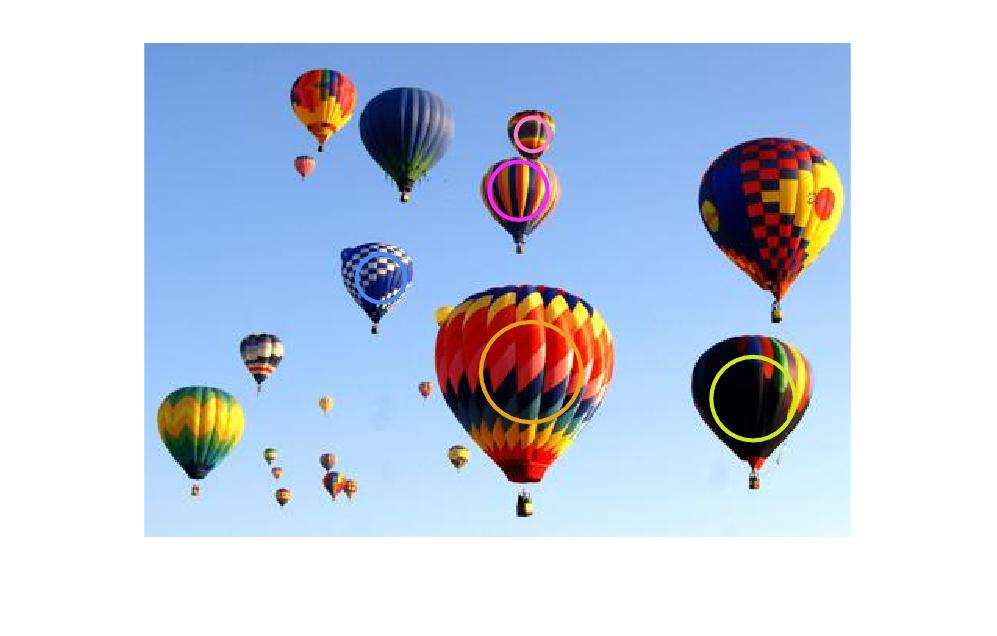
\includegraphics[width=8cm]{balloons1.jpg}
\caption{}
\end{figure}

\begin{figure}[!htbp]
\centering
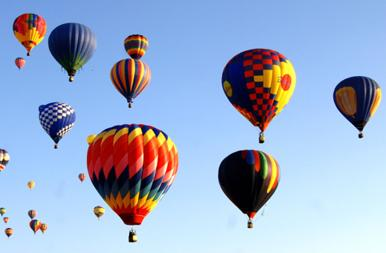
\includegraphics[width=8cm]{balloons2.jpg}
\caption{}
\end{figure}

For some reason, I was never able to make the circles better.

\end{proof}

\begin{problem}
\normalfont
Problem 2
\end{problem}


\begin{proof}

\begin{figure}[!htbp]
\centering
\includegraphics[width=15cm]{p3_page1.jpg}
\caption{This page shows picture of part of the work done for part 1 of the problem}
\end{figure}

\begin{figure}[!htbp]
\centering
\includegraphics[width=15cm]{p3_2.jpg}
\caption{This page shows picture of part of the work done for part 1 of the problem}
\end{figure}

\begin{figure}[!htbp]
\centering
\includegraphics[width=15cm]{p3_page3.jpg}
\caption{This page shows picture of part of the work done for part 1 of the problem}
\end{figure}

\begin{figure}[!htbp]
\centering
\includegraphics[width=15cm]{p3_page4.jpg}
\caption{This page shows picture of part of the work done for part 1 of the problem, particularly shows the final transform of the matrix}
\end{figure}


\begin{figure}[!htbp]
\centering
\includegraphics[width=15cm]{p3_page5.jpg}
\caption{This page shows picture of part of the work done for part 1 of the problem, particularly shows the required basis}.
\end{figure}

\begin{figure}[!htbp]
\centering
\includegraphics[width=15cm]{p3_page6.jpg}
\caption{This page shows picture of part of the work done for part 2 of the problem}
\end{figure}

\begin{figure}[!htbp]
\centering
\includegraphics[width=15cm]{p3_page7.jpg}
\caption{This page shows picture of part of the work done for part 2 of the problem, particularly shows the final reconstruction obtained.}
\end{figure}


\begin{figure}[!htbp]
\centering
\includegraphics[width=15cm]{p3_page8.jpg}
\caption{This page shows picture of part of the work done for part 3 of the problem}
\end{figure}

\begin{figure}[!htbp]
\centering
\includegraphics[width=15cm]{p3_page9.jpg}
\caption{This page shows picture of part of the work done for part 3 of the problem, particularly, shows the upper bound}.
\end{figure}

Finally, for the last part 4) of the problem. 



\end{proof}

\begin{problem}
\normalfont
Problem 3
\end{problem}

\begin{proof}
FOr this problem for both cases the MNIST and SVHN we are using 10 eigenbasis.
\begin{enumerate}

\item The following images are the first 10 eigenfaces of the problem

\begin{figure}[!htbp]
\centering
\includegraphics[width=8cm]{base0.jpg}
\caption{This is base 0}.
\end{figure}


\begin{figure}[!htbp]
\centering
\includegraphics[width=8cm]{base1.jpg}
\caption{This is base 1}.
\end{figure}

\begin{figure}[!htbp]
\centering
\includegraphics[width=8cm]{base2.jpg}
\caption{This is base 2}.
\end{figure}

\begin{figure}[!htbp]
\centering
\includegraphics[width=8cm]{base3.jpg}
\caption{This is base 3}.
\end{figure}

\begin{figure}[!htbp]
\centering
\includegraphics[width=8cm]{base4.jpg}
\caption{This is base 4}.
\end{figure}

\begin{figure}[!htbp]
\centering
\includegraphics[width=8cm]{base5.jpg}
\caption{This is base 5}.
\end{figure}

\begin{figure}[!htbp]
\centering
\includegraphics[width=8cm]{base6.jpg}
\caption{This is base 6}.
\end{figure}

\begin{figure}[!htbp]
\centering
\includegraphics[width=8cm]{base7.jpg}
\caption{This is base 7}.
\end{figure}

\begin{figure}[!htbp]
\centering
\includegraphics[width=8cm]{base8.jpg}
\caption{This is base 8}.
\end{figure}

\begin{figure}[!htbp]
\centering
\includegraphics[width=8cm]{base9.jpg}
\caption{This is base 9}.
\end{figure}



\item FOr the SVHN data set, the following image was predicted to be 202.

\begin{figure}[!htbp]
\centering
\includegraphics[width=10cm]{SVHN_wrong_image.jpg}
\caption{This page shows picture of part of the work done for part 3 of the problem, particularly, shows the upper bound}.
\end{figure}

For the MNIST data set, the following image was predicted to be 5

\begin{figure}[!htbp]
\centering
\includegraphics[width=10cm]{MNIST_wrong_image.jpg}
\caption{}.
\end{figure}

\item Finally, the error rate for the MNIST code is 72\% and the error rate for the SVHN is 97\%.

\item The code is uploaded to canvas.

\end{enumerate}

\end{proof}

\end{document}